\documentclass[12pt,a4paper]{article}
\usepackage[utf8]{inputenc}
\usepackage[spanish]{babel}
\usepackage{amsmath}
\usepackage{amsfonts}
\usepackage{amssymb}
\usepackage{graphicx}
\usepackage[left=2cm,right=2cm,top=2cm,bottom=2cm]{geometry}
\author{Enciso Guerrero Benjamin Salvador\\
Carlos Enrrique Moran Garabito\\
Cinematica De Robots }
\title{CINEMATICA DIRECTA E INVERSA DE MANIPULADORES SERIALES}
\begin{document}
\maketitle

\includegraphics[scale=1.8]{upzmgg.jpg} 
\newpage
CINEMATICA DIRECTA E INVERSA DE MANIPULADORES SERIALES.
\\\\
Presenta una articulación con movimiento rotacional y dos angulares. Aunque el brazo articulado puede realizar el movimiento llamado interpolación lineal (para lo cual requiere mover simultáneamente dos o tres de sus articulaciones), el movimiento natural es el de interpolación por articulación, tanto rotacional como angular. \\\\
Se denomina cinemática directa a una técnica que es utilizada en gráficos 3D por computadora, para solucionar y calcular la posición de partes de una estructura articulada a partir de sus elementos fijos y las transformaciones que se provocan por las articulaciones de la estructura. \\\\
La cinemática inversa se refiere a la utilización de las ecuaciones cinemáticas de un robot para determinar los parámetros comunes que proporcionan una posición deseada del efector final. Especificación del movimiento de un robot de manera que su extremo efector logra una tarea deseada es conocido como planificación de movimientos. La cinemática inversa transforma el plan de movimiento en trayectorias del actuador en conjuntos para el robot. \\\\

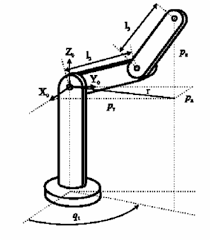
\includegraphics[scale=1.5]{images.png} 
\\\\
Robot antropomorfico con 3 grados de livertad. \\\\
el robot se moverá en X y Y, así realizando los movimientos que se les indiquen ya que este se le colocara las pinzas de la soladura por encima del robot. 


\end{document}